% ---------------------------------------
%
%  Extend to SU(5) GUT
%  extend_SU5.tex
%  Program modified by Yasutoki Takamura
%  Last Modified Jan 27 2025
%
% ---------------------------------------
ここまでで$SU(5)$大統一理論について見ることができた.
電荷の量子化を理論に基づいて自然と説明されることは$SU(5)$大統一理論の魅力的な点である.
一方で, 陽子崩壊やワインバーグ角など現在の実験と整合性の合わない事実も残される.
さらに標準模型の課題を$SU(5)$大統一理論によってすべて解決することができない.
そのため, 高いエネルギースケールで3つの相互作用が統一されるべきという立場を取るならば, 大統一理論を拡張し, 標準模型を超えた物理を探査することが必要となる.

したがって, ここまで見てきたH.Georgi, S.L.Glashowによる$SU(5)$大統一模型を最小$SU(5)$模型と呼び, 最小$SU(5)$模型の課題と, その拡張方法として高次元のヒッグス粒子を仮定する例を考える.
\section{最小SU(5)大統一理論の課題}
最小$SU(5)$大統一理論について, 予言と課題については前節で述べた.
ここでは, 標準模型のもつ理論の課題と, 大統一理論の課題について両方の立場でどのように考えられるかを簡単に述べる.
\begin{itemize}
  \item ゲージ結合定数の統一\\
        くりこみ群方程式を解くことにより, ゲージ結合定数の大きさのエネルギー依存性を求めることができた.
        大統一理論は高いエネルギースケールではゲージ結合定数は1つに統一されるべきであると考える.
        ところが図\ref{fig:RGE_SM}で見たように, 最小$SU(5)$大統一理論ではゲージ結合定数の大きさは統一されない.
  \item ニュートリノ質量\\
        標準模型を拡張して重たい場を加えてニュートリノ質量を導く方法はあるが, 大統一理論はそのような拡張よりも高いエネルギースケールで成り立つ理論である.
        そのため, 大統一スケールであればそのような拡張を自然と含んだ模型である必要がある.
        最小$SU(5)$大統一理論は標準模型粒子の他に, $T \,(\in \phi_{\bar{\bm{5}}})$ヒッグスと$X,Y$ボゾンを含むが, 右巻きのカイラリティを持つニュートリノ$\nu_R$を含まないため, ニュートリノのディラック型質量項を表すことができない. 
\end{itemize}
場の量子論に基づくと, ゲージ対称性により許される表現は理論に加えることが可能である.
ここでは高次元表現で表される粒子による拡張を与え, それらが現象論的にどのような予言をもたらすのか次節から考える.
\section{45表現ヒッグスを用いた拡張}
大統一理論において, 式(\ref{decon_510})のように基本表現である$\bm{5}$表現から$\bm{45}$表現を構成することができる.
この表現を用いた$\bm{45}$表現ヒッグス$(\phi_{\bm{45}})$ を考え, 
最小$SU(5)$模型で予言された下系列クォークと荷電レプトンの質量比についての予言$M_d = M_e$に修正を行うことができる
\cite{framptonEstimateFlavorNumber1979,georgiNewLeptonquarkMass1979}.
$\bm{45}$表現ヒッグスは
\begin{align}
  \left(\phi_{\bm{45}}\right)^{ij}_k = -(\phi_{\bm{45}})^{ji}_k,\quad (\phi_{\bm{45}})^{ij}_i =0 \quad(i,j,k =1,\cdots,5)\nonumber
\end{align}
と
また, $\phi_{\bm{45}}$は次のように分解される.
\begin{align}
  \phi_{\bm{45}} &= \varphi_8 \left(\bm{8}, \bm{2}, \frac{1}{2}\right) \oplus \varphi_{\bar{6}}\left(\overline{\bm{6}}, \bm{3}, -\frac{1}{3}\right) \oplus \varphi_3^T\left(\overline{\bm{3}}, \bm{3}, -\frac{1}{3}\right) \nonumber\\
                 &\qquad\qquad\oplus \varphi_3^D\left( \overline{\bm{3}}, \bm{2}, -\frac{7}{6}\right) \oplus \varphi_3^S\left(\bm{3}, \bm{1}, -\frac{1}{3}\right)\oplus \varphi_{\overline{3}}^S\left( \overline{\bm{3}}, \bm{1}, \frac{4}{3}\right)\oplus H_2\left(\bm{1}, \bm{2}, \frac{1}{2}\right)\nonumber
\end{align}
湯川結合は次のようになる.
\begin{align}
  (\psi_{\bm{\bar{5}}La}^T)_a C (\psi_{\bm{10}L})^{bc} (\phi_{\bm{45}}^\dagger)_{bc}^a+\mathrm{h.c.}\label{Y_45a}\\
  \varepsilon_{abcef} (\psi_{\bm{10}L}^T)^{ab} C (\psi_{\bm{10}L})^{cd} (\phi_{\bm{45}})_d^{ef}+ \mathrm{h.c.}\label{Y_45b}
\end{align}
$\bm{45}$表現ヒッグスは真空期待値を
\begin{align}
  \langle (\phi_{\bm{45}})^{j5}_i\rangle = v_{45}\left(\delta^j_i - 4\delta^j_4 \delta_i^4\right),\quad(i,j=1,\cdots 4)
\end{align}
と取ることにより, ゲージ対称性を$SU(3)_c\times U(1)_{em}$へ破る.
このとき, 式(\ref{Y_45a})(\ref{Y_45b})より質量行列が
\begin{align}
  M^e_{45} = -3M_{45}^d
\end{align}
となり, $\bm{5}$表現ヒッグスとは異なる結果となる.

\section{15表現ヒッグスを用いた拡張}
ニュートリノ質量を生成する機構はいくつか考えられている.
その中で, タイプIIシーソー機構によってニュートリノ質量を説明するためには$SU(2)_L$三重項のスカラー粒子が理論に含まれている必要がある.

$SU(5)$対称性において, ヒッグス粒子を$\bm{15}$表現で導入した場合, ラグランジアンに$SU(2)_L$三重項のスカラー粒子を含めることができる\cite{dorsner_phenomenological_2006,dorsner_unification_2005}.
$\bm{15}$表現ヒッグスを$\phi_{\bm{15}}$と書き, 次のように分解することができる\footnote{この記法は\cite{dorsnerPhysicsLeptoquarksPrecision2016}を参考にした.}.
\begin{align}
  \phi_{\bm{15}} = \Delta \left(\bm{1}, \bm{3}, 1\right) \oplus \widetilde{R_2}\left(\bm{3}, \bm{2},\frac{1}{6}\right)\oplus S\left(\overline{\bm{6}}, \bm{1}, -\frac{2}{3}\right)
\end{align}
一般的に行列で表した場合は
\begin{align}
  \phi_{\bm{15}} = \begin{pmatrix}
    S & {\widetilde{R_2}} \\
    \widetilde{R_2}^T & \Delta
  \end{pmatrix}
\end{align}
となる.
$\bm{15}$表現ヒッグスはフェルミオンと次のように湯川結合をする.
\begin{align}
  \Delta\mathcal{L}_Y = \overline{\psi_{\bm{\bar{5}}}} Y_{15} \phi_{\bm{15}}\overline{\psi_{\bm{\bar{5}}}} 
\end{align}
ここで, $\Delta$が真空期待値$v_\Delta$を持つとすると, シーソー機構のラグランジアンは
\begin{align}
  -M_\Delta^2 \mathrm{Tr}(\Delta^\dagger \Delta) + Y_{15} L\Delta L +c \phi_{\bm{5}}\Delta^\dagger \phi_{\bm{5}} +\mathrm{h.c.}\nonumber
\end{align}
これは通常のタイプIIシーソー機構と同じラグランジアンである.
真空期待値をとることで
\begin{align}
  m_\nu \simeq \frac{Y_{15}}{M_\Delta^2}v_{15}^2\nonumber
\end{align}
とニュートリノ質量を与える.

$\bm{15}$表現ヒッグスに含まれる$S$はレプトクォークであり, 次のような相互作用項が含まれる.
\begin{align}
  \mathcal{L}_{\mathrm{int}} = d^c Y_15 S L\nonumber
\end{align}
したがって, この相互作用によって陽子崩壊が起こるため, 大統一スケールよりも低いエネルギースケールに存在してしまうと頻繁に陽子が崩壊してしまう.
そのため, このスカラー粒子$S$が存在するエネルギースケールは任意であることを用いて, 大統一スケールよりも高いスケールに存在すると仮定することが多い.

\subsection{15表現ヒッグスを用いた大統一}
ここで実際に新たな粒子を仮定して繰り込み群方程式を解くことを考える.
$\bm{15}$表現ヒッグスが持つくりこみ群方程式の係数$b_i=(b_1, b_2, b_3)$は
\begin{align}
  b_i^\Delta=\begin{pmatrix}
    \cfrac{3}{5} & \cfrac{2}{3} & 0
  \end{pmatrix},\qquad
  b_i^{\widetilde{R_2}}=\begin{pmatrix}
    \cfrac{1}{30} & \cfrac{1}{2} & \cfrac{1}{3}
  \end{pmatrix},\qquad
  b_i^{S}=\begin{pmatrix}
    \cfrac{8}{15} & 0 & \cfrac{5}{6}
  \end{pmatrix}
\end{align}
である.

先に述べてあるようにレプトクォーク$S$は低いエネルギースケールに存在すると陽子崩壊を頻繁に起こしてしまうため, $S$は大統一スケール以上に存在すると仮定する.
一方で, 電弱スケールと大統一スケールの間には$\Delta, \widetilde{R_2}$の2つの粒子が存在すると仮定する.
また, 2つの粒子が階層性を持つことを仮定することで大統一をよりよく行えるようにする.
図\ref{fig:RGE_15_1loop}は実際に繰り込み群方程式を1次の量子補正まで含めて解いた図である.
\begin{figure}[ht]
  \centering
  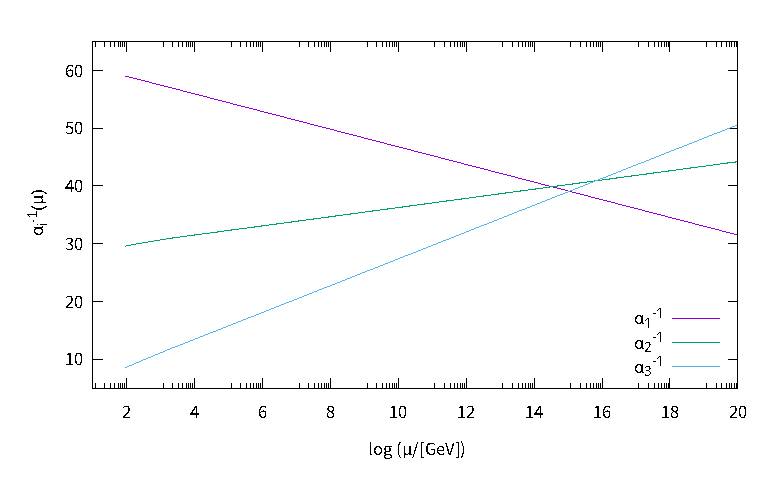
\includegraphics[width=12truecm,clip]{fig/RGE_15_1loop.eps}
  \caption{$\bm{15}$表現ヒッグスを加えた場合の走る結合定数. $M_\Delta=1.54\,[\mathrm{TeV}]$, $M_{\widetilde{R_2}}=250\,[\mathrm{GeV}]$ }
  \label{fig:RGE_15_1loop}
\end{figure}

標準模型粒子のみ用いた図\ref{fig:RGE_SM}は大統一スケール付近では結合定数は統一されなかった.
$\bm{15}$表現ヒッグスに対して行った階層性の仮定を, $M_\Delta = 1.54[\mathrm{TeV}]$, $M_{\widetilde{R_2}} =250\,[\mathrm{GeV}]$とすることで, 標準模型よりもよりゲージ結合定数の大きさが近づくことがわかる.

%EOF
